\documentclass{standalone}

\usepackage{tikz}
\usetikzlibrary{arrows.meta, decorations.markings}

\tikzset{
    midarrow/.style={
        decoration={markings, mark=at position 1 with {\arrow{Latex}}},
        postaction={decorate}
    }
}

\begin{document}

	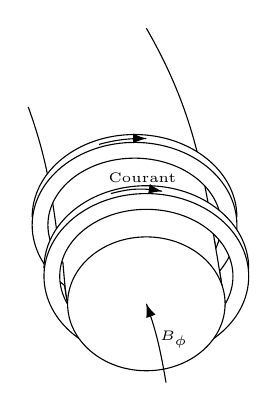
\begin{tikzpicture}
    
    \draw
    (-1.5,2.5)
    to [out=-70, in=100]
    (-1,0);
    
    \draw
    (0,3.5)
    to [out=-60, in=100]
    (1, 0);
    
    % Deuxième bobine
    
    \fill[white]
        (1.1-0.15,1) [x radius=1.1cm, y radius=0.85cm] arc[start angle=0, end angle=360]
        (1.3-0.15,1) [x radius=1.3cm, y radius=1.05cm]   arc[start angle=360, end angle=0]
        -- cycle;
        
     % paramètres : centre (cx,cy), grand rayon (Rx,Ry), petit rayon (rx,ry)
  \def\cx{-0.15}   % = 1.3-0.15
  \def\cy{1.1}
  \def\Rx{1.30}
  \def\Ry{1.05}
  \def\rx{1.10}   % rayon intérieur légèrement plus petit
  \def\ry{0.85}

  \fill[white]
    (\cx+\Rx,\cy)
      arc[start angle=0, end angle=180, x radius=\Rx, y radius=\Ry]
    -- (\cx-\rx,\cy)
      arc[start angle=180, end angle=0, x radius=\rx, y radius=\ry]
    -- cycle;
        
	\draw (-0.15,1) ellipse [x radius=1.1cm, y radius=0.85cm];

	\draw (-0.15,1) ellipse [x radius=1.3cm, y radius=1.05cm];    

	\draw (1.3-0.15,1.1) [x radius=1.3cm, y radius=1.05cm] 
    arc[start angle=0, end angle=180];

	% Premi_re bobine
    
    \fill[white]
        (1.1,0.35) [x radius=1.1cm, y radius=0.85cm] arc[start angle=0, end angle=360]
        (1.3,0.35) [x radius=1.3cm, y radius=1.05cm]   arc[start angle=360, end angle=0]
        -- cycle;
        
    \def\cy{0.45}
    \def\cx{0}
        
          \fill[white]
    (\Rx,\cy)
      arc[start angle=0, end angle=180, x radius=\Rx, y radius=\Ry]
    -- (\cx-\rx,\cy)
      arc[start angle=180, end angle=0, x radius=\rx, y radius=\ry]
    -- cycle;
    
    \draw (1.3,0.45) [x radius=1.3cm, y radius=1.05cm] 
    arc[start angle=0, end angle=180];
        
        \draw (0,0.35) ellipse [x radius=1.1cm, y radius=0.85cm];

	\draw (0,0.35) ellipse [x radius=1.3cm, y radius=1.05cm];
	
	% Correction de la bobine arrière
	\fill[white]
		(-1.06,0.53)	 to [out=-85, in=100]
    (-1,0) -- (1, 0) to [out=100, in=-80] (0.86, 0.83) -- cycle;
	
    \draw
    (-1.06,0.53)
    to [out=-85, in=100]
    (-1,0);
    
    \draw
    (0.86,0.83)
    to [out=-80, in=100]
    (1,0);
    
    % Centre du tokamak
    \draw[fill=white] (0,0) ellipse [x radius=1cm, y radius=0.85cm];
    
    \draw[midarrow]
    (0.25, -1)
    to [out=100, in=-70]
    (0,0);
    
    \draw[midarrow]
    (-0.6, 2.025)
    to [out=15, in=180]
    (0,2.1);
    
    \draw[midarrow]
    (-0.45, 1.4)
    to [out=15, in=170]
    (0.2, 1.43);
    
    \node at (-0.05, 1.6) {\tiny Courant};
    \node at (0.35, -0.45) {\tiny \( B_\phi \)};
	
	\end{tikzpicture}

\end{document}